\documentclass[12pt]{report}

\usepackage[a4paper, total={6in, 9in}]{geometry}
\usepackage{tikz}
\usepackage{array}
\usepackage{amsthm}
\usepackage{courier}
\usepackage{titlesec}
\usepackage{graphicx}
\usepackage{multibib}
\usepackage{hyperref}
\usepackage{pgfplots}
\usepackage{algorithm2e}

\hypersetup{colorlinks=true, citecolor=black, linkcolor=black, urlcolor=blue}
\newcolumntype{L}[1]{>{\raggedright\let\newline\\\arraybackslash\hspace{0pt}}m{#1}}
\newcolumntype{C}[1]{>{\centering\let\newline\\\arraybackslash\hspace{0pt}}m{#1}}
\newcolumntype{R}[1]{>{\raggedleft\let\newline\\\arraybackslash\hspace{0pt}}m{#1}}
\titleformat{\chapter}[display] {\normalfont\Huge\bfseries}{\chaptertitlename\ \thechapter}{0pt}{\Huge}
\titlespacing{\chapter}{0cm}{0cm}{1cm}
\counterwithout{figure}{chapter}
\counterwithout{table}{chapter}
\pgfplotsset{compat=1.18}
\theoremstyle{definition}
\newtheorem*{example}{Example}
\theoremstyle{definition}
\newtheorem*{algo}{Algorithm}
\theoremstyle{definition}
\newtheorem*{method}{Method}
\RestyleAlgo{ruled}



\begin{document}



\begin{titlepage}
    \newcommand{\HRule}{\rule{\linewidth}{0.5mm}} %Horizontal line break%
    \center
    \textsc{\LARGE Université Toulouse III Paul Sabatier}\\[2.5cm]
    \textsc{\Large Master Thesis Report}\\[0.5cm]
    \textsc{\large Computer Science for Aerospace}\\[2.5cm]

    \HRule\\[0.5cm]
    {\huge \bf Multivariate Decision Tree Classification}\\[0.5cm]
    \HRule\\[1.5cm]

    \begin{minipage}{0.4\textwidth}
		\begin{flushleft}
			\large
			\textit{Author}\\
			Dany Morales
		\end{flushleft}
	\end{minipage}
    \begin{minipage}{0.4\textwidth}
		\begin{flushright}
			\large
			\textit{Supervisors}\\
			Martin Cooper\\
            Emmanuel Hebrard
		\end{flushright}
	\end{minipage}

    \vfill
    \large January 2024

    
\includegraphics[width=0.5\textwidth]{logo.png}
\end{titlepage}



\tableofcontents



\chapter*{Introduction}
\paragraph{} This report is about the work achieved during the thesis in the second year of master in Computer
Science for Aerospace. The supervisors are Mr. Martin Cooper at the \textit{Institut de Recherche en Informatique
de Toulouse (IRIT)} and Mr. Emmanuel Hebrard at the \textit{Laboratoire d'Analyse et d'Architecture des Systèmes
in Toulouse (LAAS)}. This is a direct continuation of our work done during the TER of summer 2023, in which we
implemented our own version of a heuristic algorithm for multivariate decision tree classification. This time,
we will work with an algorithm named \texttt{Blossom} which is an optimal decision tree classification algorithm
created in part by Mr. Hebrard. The goal of this master thesis is to find a way for this algorithm to support
multivariate decision trees. We will first introduce useful notions related to this topic with a brief state
of the art on decision tree classification. Afterwards, we will present what we have done so far and some
results we have obtained. Finally we will overview what we are planning for the rest of the thesis.



\chapter{Preliminary research}
\section{Decision trees}
\paragraph{} A decision tree is a type of tree that helps to make a choice given a certain problem. In figure
\ref{fig:tree}, the problem would be if it is possible to go play outside depending on the weather.

\begin{figure}[ht]
    \centering
    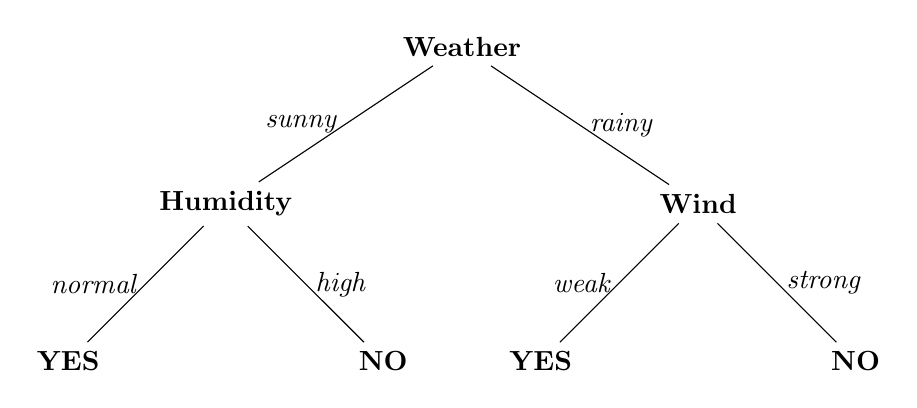
\begin{tikzpicture}
        [
            level 1/.style = {level distance = 2cm, sibling distance = 6cm},
            level 2/.style = {sibling distance = 4cm}
        ]
        
        \node {\bf Weather}
            child {node {\bf Humidity}
            child {node {\bf YES}
            edge from parent node [left] {\it normal}}
            child {node {\bf NO}
            edge from parent node [right] {\it high}}
            edge from parent node [left] {\it sunny}} 
            child {node {\bf Wind}
            child {node {\bf YES}
            edge from parent node [left] {\it weak}}
            child {node {\bf NO}
            edge from parent node [right] {\it strong}}
            edge from parent node [right] {\it rainy}};
    \end{tikzpicture}
    \caption{``\textit{Play outside}'' decision tree}
    \label{fig:tree}
\end{figure}

\paragraph{} This decision tree is the result of the classification of the dataset in figure \ref{fig:dataweather}.

\begin{table}[ht]
    \centering
    \begin{tabular}{||c c c c||} 
    \hline
    Weather & Humidity & Wind & Play\\[0.5ex]
    \hline\hline
    Sunny & High & Strong & NO\\ 
    Sunny & Normal & Strong & YES\\
    Rainy & High & Strong & NO\\
    Rainy & High & Weak & YES\\ 
    \hline
    \end{tabular}
    \caption{``\textit{Play outside}'' dataset}
    \label{fig:dataweather}
\end{table}

\paragraph{} According to this decision tree, if it is sunny and the humidity is normal, we can play outside.
On the other hand, if there is rain and wind, we cannot play outside. Weather, humidity and wind are called
features. This tree has two outcomes also called classes: YES and NO. On each node or decision node, the dataset
is split into two subsets depending on a chosen feature. At the root, we split on the weather feature: each
value of the dataset with $weather = sunny$ will be on the left subtree and each value of the dataset with
$weather = rainy$ will be on the right subtree.


\section{Classification concepts}
\paragraph{} A decision tree can be built from a dataset, the root node represents the entire set, then it is
divided into two more homogeneous sets creating two new decision nodes. We repeat this process recursively
until a specified maximum depth or until the subset is considered \textbf{pure}.

\paragraph{} The purify of a set can be defined with several metrics. A naïve way of defining it would be for
example, in a set in which there is a gender feature composed of 70\% males and 30\% females, the purity of
the set would be 70\%. We will introduce two methods used to find the purity of a set used in various algorithms.

\begin{method}[Information gain]
    The information gain uses the entropy in order to establish the purity of two subsets. If the information
    gain is high, the two subsets are considered pure, on the contrary, low information gain means impure
    subsets.
    \begin{displaymath}
        InformationGain(S) = H(S) - [H(S_1) + H(S_2)]
    \end{displaymath}
    \paragraph{} $S_1$ and $S_2$ are the two subsets resulting from spliting $S$. The entropy $H$ of a set $S$
    with $J$ classes can be defined using the Shannon entropy where $p_i$ is the probability of the class $i$
    to happen.
    \begin{displaymath}
        H(S) = - \sum_{i=1}^{J} p_i log_2 p_i
    \end{displaymath}
    \paragraph{} This means that a set with a large entropy is not pure meanwhile a small entropy signifies a
    better purity. A set with an entropy of zero is pure i.e. only one class is remaining which also means this
    is a leaf in the decision tree. If a split is good, $S_1$ and $S_2$ will have a small entropy compared to the
    parent set $S$ thus the information gain will be high.
\end{method}

\begin{method}[Gini impurity]
    An another way of computing the purity of set is using the Gini index. It measures the probability for a
    random element of the set to be misclassified.
    \begin{displaymath}
        G(S) = 1 - \sum_{i=1}^{J} p_i^2
    \end{displaymath}
    \paragraph{} A value of zero means that all instances of a set have the same class i.e. the set is pure.
    When spliting a set, we must do a weighted average of the Gini index for every subset. If this average is lower
    than the Gini index of the parent set, this means the split is good.
\end{method}

\paragraph{} Both these methods are viable and provide different results depending on the implementation but
the choice of impurity measurement can have a significant impact. Other indicators exist such as variance 
reduction or chi-square however, the algorithms we will consider mainly use information gain and Gini index.


\section{Multivariate decision trees}
\paragraph{} ``A multivariate decision tree is a decision tree in which the condition tested at a node is a 
constraint on any number of features \cite{multivariate-explaining}.'' The principles of information gain,
entropy and Gini impurity are still valid but, as we introduce another condition to test, finding the best
split for each decision node becomes more costly to compute.

\begin{figure}[ht]
    \centering
    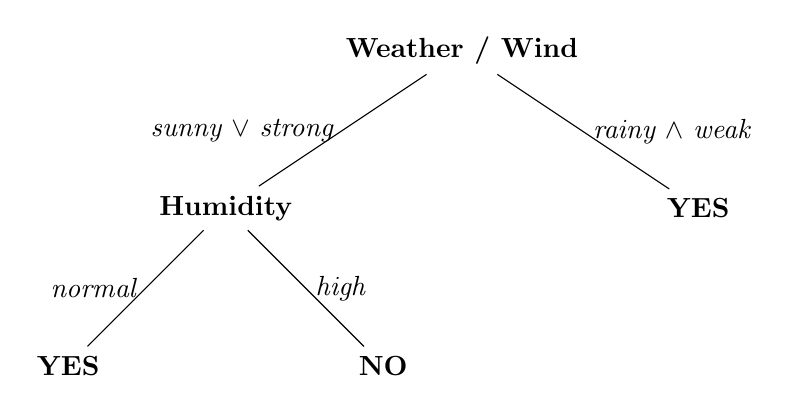
\begin{tikzpicture}
        [
            level 1/.style = {level distance = 2cm, sibling distance = 6cm},
            level 2/.style = {sibling distance = 4cm}
        ]
        
        \node {\bf Weather / Wind}
            child {node {\bf Humidity}
            child {node {\bf YES}
            edge from parent node [left] {\it normal}}
            child {node {\bf NO}
            edge from parent node [right] {\it high}}
            edge from parent node [left] {\it sunny $\lor$ strong}} 
            child {node {\bf YES}
            edge from parent node [right] {\it rainy $\land$ weak}};
    \end{tikzpicture}
    \caption{``\textit{Play outside}'' multivariate decision tree}
    \label{fig:multitree}
\end{figure}

\paragraph{} This is a possible multivariate decision tree that classifies the dataset in figure \ref{fig:dataweather}.
The root node test condition is on both the weather and wind features. The left child contains the subset
satisfying the condition $(weather=sunny \lor wind=strong)$ and the right child contains the subset satisfying
the negation i.e. $(weather=rainy \land wind=weak)$. It is important to note that the number of features a
condition is testing do not have to be the same at every node.



\chapter{State of the art}
\section{Decision tree learning} 
\paragraph{} Decision tree learning is a supervised learning method used in machine learning. An optimal tree i.e.
the tree with the best accuracy given a dataset is not easy to find using heuristic algorithms since this is
a NP-hard problem. As a consequence, most heuristic algorithms use a greedy approach with sometimes pruning
done to remove unecessary branches to achieve better accuracy.

\paragraph{} A classical greedy approach iterates over every feature and for each feature is considered every
value as a possible split, once the best split is found, the tree grows and it recursively continues.
Such an approach has a time complexity at every decision node of $O(\sum_{i}^{}F_i)$ where $F_i$ is the number
of distinct values for the feature $i$. The worst-case scenario being $O(mn)$ where $m$ is the number of
features and $n$ is the number of instance in the set. In a multivariate decision tree, we introduce an
additional condition to test at every node so the time complexity becomes $O(\sum_{i}\sum_{j}F_iF_j)$ which at
worst is $O(m^2n^2)$.

\paragraph{} The version of \texttt{ID3} we implemented during our TER as well as the following heuristic methods have
comparable worst-case time complexities in addition of not finding optimal trees.
%complexity comparison table?%

\newpage

\section{Heuristic algorithms}
\begin{algo}[\texttt{ID3}]
    Iterative Dichotomiser (1986) is a greedy algorithm developed by Ross Quilan that splits the dataset
    using the information gain metric. This algorithm is the one we implemented and adapted in Python during
    our TER.\\
    $\mathcal{D}$ is the input dataset and $\mathcal{F}$ contains the features of a given set.

    \begin{algorithm}
        \caption{\texttt{ID3}}\label{alg:two}
        \DontPrintSemicolon
        \KwData{$\mathcal{D}$, $depth_{max}$}
        \SetKwFunction{BuildTree}{BuildTree}
        \SetKwFunction{BestSplit}{BestSplit}

        \SetKwProg{Bn}{Function}{:}{}
        \Bn{\BuildTree{$S, depth=0$}}{
            \If{$depth \leq depth_{max}$}{
                $(left, right) \gets \BestSplit{S}$\;
                $subtree_L \gets \BuildTree{left, depth+1}$\;
                $subtree_R \gets \BuildTree{right, depth+1}$\;
                \KwRet $Node(subtree_L, subtree_R)$
            }
            \KwRet $Leaf(S)$\;
        }
        \;
        \SetKwProg{Sn}{Function}{:}{}
        \Sn{\BestSplit{$S$}}{
            $IG \gets 0$

            \ForEach{$f \in \mathcal{F}$}{
                $\mathcal{T} \gets thresholds(f)$

                \ForEach{$t \in \mathcal{T}$}{
                    $(l, r) \gets split(S, t, f)$

                    \If{$IG \neq \max(IG, infogain(S, l, r))$}{
                        $(left, right) \gets (l, r)$\;
                        $IG \gets infogain(S, l, r)$
                    }
                }
            }
            \KwRet $(left, right)$
        }
        \;

        \BuildTree{$\mathcal{D}$}
    \end{algorithm}

    \begin{itemize}
        \item $thresholds(f)$ gives all the possible values of a feature $f$
        \item $split(S, t, f)$ splits the dataset $S$ at the treshold value $t$ on the feature $f$
        \item $infogain(S, l, r)$ computes the information gain of the split, so the set $S=l+r$ 
    \end{itemize}
\end{algo}

\begin{algo}[\texttt{C4.5}]
    Developed in 1993 by Ross Quilan, it is the successor of \texttt{ID3} and works the same way. It is an extension
    of \texttt{ID3} offering several improvements. This version can handle both continuous and discrete values.
    Some post processing is added called pruning: it eliminates branches that do not provide additional
    information. Further versions of this algorithm have been made mainly for performance improvements but
    the core principle stays the same.
\end{algo}

\begin{algo}[\texttt{CART}]
    Classification and Regression Trees, similarly to \texttt{ID3} and \texttt{C4.5} separates the data at each node
    on a given threshold and recursively iterates. It also supports continuous and discrete values. Unlike the algorithms
    above, \texttt{CART} uses the Gini impurity measure to split the dataset. Trees are grown to their maximal size
    without stopping rules then, cost-complexity pruning is done which is a more advanced pruning technique
    than the one used by \texttt{C4.5}.
\end{algo}


\section{Optimal algorithms}
\begin{algo}[\texttt{DL8}]
\end {algo}

\begin{algo}[\texttt{MurTree}]
\end {algo}

\begin{algo}[\texttt{Blossom}]
\end {algo}



\chapter{Actual work}
\section{Objective and expected results} %explain the structure of the datasets%
\paragraph{} The objective of this master thesis is to adapt the \texttt{Blossom} algorithm to support multivariate
decision trees. Since \texttt{Blossom} is an anytime algorithm, even with a very large dataset and many features,
we can always expect a result compared to a traditional heuristic algorithm, thus \texttt{Blossom} seems particularly
adapted for experimenting on MDT's. To achieve this, we have thought about several approaches: modify the
input datset file (preprocessing approach) or change the algorithm code itself (algorithmic approach).
Depending on the size of the dataset, we expect varying results. On a smaller dataset, given enough
processing time, we expect to have optimal MDT's. However, on very large datasets, adding all the feature
combinations will probably cause the algorithm to reach the maximum time chosen and interrupt the execution.
It is important to note that the preprocessing approach is not intended to be used on massive datasets as
the number of added features will become too unreasonable, creating files several gigabytes in size,
too tedious to work with. 


\section{Preprocessing approach}
\paragraph{} For the preprocessing approach, we made a simple python script to expand the features of a binary
dataset. The script can add new features of value $a \lor b$ for each possible combination of two distinct
features a and b present in the inital dataset.

\begin{example}
    For a dataset containing four features $a$, $b$, $c$ and $d$, the script will add the following six new
    features: $a \lor b$, $a \lor c$, $a \lor d$, $b \lor c$, $b \lor d$, $c \lor d$.
\end{example}

\paragraph{} The number of new features added is $k$ $n \choose 2$ where $n$ is the number of features in
the initial dataset and $k$ is the number of cnfs used. The other supported cnfs are $(\neg x \lor y)$,
$(x \lor \neg y)$, $(\neg x \lor \neg y)$, $(x \oplus y)$. The script allows to expand a dataset with any number
of cnfs chosen. The expanded dataset is given in output and is directly ready to use with the \texttt{Blossom} algorithm.
It is important to note we do not do extra preprocessing to verify if two features have the same values since
\texttt{Blossom} already has some preprocessing steps, including feature reduction that would eliminate any unecessary or
redundant feature.


\section{Other approaches}
\paragraph{} The approach we first thought about was to directly alter the code of \texttt{Blossom}. Although the
algorithm is fairly simple to understand, the code is quite complex and written in C++, have no experience in
this language, we decided to start with the preprocessing approach as a proof of concept.

\paragraph{} In the second part of the master thesis we have a few possibilities:

\begin{itemize}
    \item further improve our preprocessing algorithm to try and eliminate unecessary features to support bigger
    datasets
    \item find the abductive explanation \cite{multivariate-explaining} of the output multivariate decison trees
    from \texttt{Blossom} in order to obtain the same decisions with smaller trees
\end{itemize}



\chapter{Analysis}
\section{Discussion}
\paragraph{} In order to test how our expanded datasets performed, we selected 8 datasets and tested both their normal
and expanded versions (noted ex). We constrained the research to a maximum depth of 4, the maximum runtime to 15 minutes
and we use 80\% of the dataset for training and 20\% for testing. Finally, we tested those datasets using 5 different
seeds. We keep the trace of the algorithm and we compare the number of features, the feature reduction done (red.) during
preprocessing and both the accuracy and test accuracy.

\begin{table}[ht]
    \centering
    \begin{tabular}{L{3.5cm} R{1.8cm} R{1.8cm} R{1.8cm} R{1.8cm} R{1.8cm}}
        \hline
        \multicolumn{6}{c}{$seed=1$ | $max depth=4$ | $test sample=.2$ | $time=900$} \\
        \hline
        \bf dataset & \bf features & \bf red. & \bf acc. & \bf test acc. & \bf cpu \\
        \hline
        \tt anneal & 93 & 44 & 0.8859 & 0.8834 & 1.162 \\
        \tt anneal ex & 21483 & 18368 & 0.9013 & 0.8834 & 900 \\
        \tt car-un & 21 & 0 & 0.9247 & 0.8901 & 0.166 \\
        \tt car-un ex & 1071 & 126 & 0.9782 & 0.9653 & 900 \\
        \tt diabetes & 112 & 56 & 0.8257 & 0.7662 & 5.271 \\
        \tt diabetes ex & 31192 & 24212 & 0.8811 & 0.7727 & 900 \\
        \tt ionosphere & 445 & 223 & 0.9857 & 0.9014 & 565.1 \\
        \tt ionosphere ex & 494395 & 380485 & 0.9964 & 0.9436 & 900 \\
        \tt iris-bin & 12 & 3 & 0.9916 & 1.0000 & 0 \\
        \tt iris-bin ex & 342 & 235 & 0.9915 & 1.0000 & 0 \\
        \tt lymph & 68 & 22 & 0.9914 & 0.8387 & 0.463 \\
        \tt lymph ex & 11458 & 7947 & 1.0000 & 0.8387 & 900 \\
        \tt monk1-bin & 11 & 0 & 1.0000 & 0.9230 & 0.004 \\
        \tt monk1-bin ex & 286 & 24 & 1.0000 & 1.0000 & 1.078 \\
        \tt mushroom & 119 & 19 & 1.0000 & 1.0000 & 42.92 \\
        \tt mushroom ex & 35224 & 23765 & 1.0000 & 1.0000 & 900 \\
        \hline
        \bf Average & & & \bf 0.9506 & \bf 0.9003 & \\
        \hline
        \bf Average ex & & & \bf 0.9685 & \bf 0.9254 & \\
        \hline
    \end{tabular}
    \caption{Test accuracy of \texttt{Blossom} with extended datasets for $seed=1$}
    \label{fig:seedone}
\end{table}

\paragraph{} We can see in table \ref{fig:seedone} that overall, we get a better accuracy and test accuracy when using
an expanded dataset. Although during training the gain can be negligible, we get as much as a 7\% gain with some datasets 
(\texttt{car-un} and \texttt{monk1-bin}) in testing accuracy. On average, the accuracy improves by around 2\% for this
seed.

\paragraph{} For most expanded datasets, the execution reaches its time limit and is interrupted, which means the search
is not finished and it is still possible to find a more optimal tree. On the contrary, for the non-expanded datasets,
the search found the optimal tree and thus the maximum accuracy possible. By expanding these datasets, we are now able to
go past the original maximal accuracy given enough computing time.

\paragraph{} Since the total execution time can be misleading, using the same parameters, we compared the first result
of the search for each dataset. If the algorithm cannot find a first tree in less than one second, the result is
omitted which happened only for \texttt{ionosphere ex}.

\begin{table}[ht]
    \centering
    \begin{tabular}{L{3.5cm} R{1.8cm}}
        \hline
        \bf dataset & \bf first acc. \\
        \hline
        \tt anneal & 0.8351 \\
        \tt anneal ex & 0.8782 \\
        \tt car-un & 0.9015 \\
        \tt car-un ex & 0.9565 \\
        \tt diabetes & 0.7931 \\
        \tt diabetes ex & 0.8550 \\
        \tt ionosphere & 0.9285 \\
        \tt ionosphere ex & - \\
        \tt iris-bin & 0.9916 \\
        \tt iris-bin ex & 0.9915 \\
        \tt lymph & 0.9316 \\
        \tt lymph ex & 0.9829 \\
        \tt monk1-bin & 0.8979 \\
        \tt monk1-bin ex & 1.0000 \\
        \tt mushroom & 1.0000 \\
        \tt mushroom ex & 1.0000 \\
        \hline
        \bf Average & \bf 0.9099 \\
        \hline
        \bf Average ex & \bf 0.9520 \\
        \hline
    \end{tabular}
    \caption{First accuracy of the search if $time<1$}
    \label{fig:firstacc}
\end{table}

\paragraph{} When looking at the first results obtained in table \ref{fig:firstacc}, we have a 5\% average gain in
accuracy for the same execution time. This means that \texttt{Blossom} is able to find a better decision tree in the
same amount of time for the expanded datasets.

\newpage

\section{Performance}
\paragraph{} As we discussed, extended datasets provide the same or better accuracy for the same execution time as well
as allowing to continue the search for even more accuracy. We decided to investigate this behavior further, specifically
using the \texttt{anneal} dataset.

\begin{figure}[ht]
    \centering
    \begin{center}
        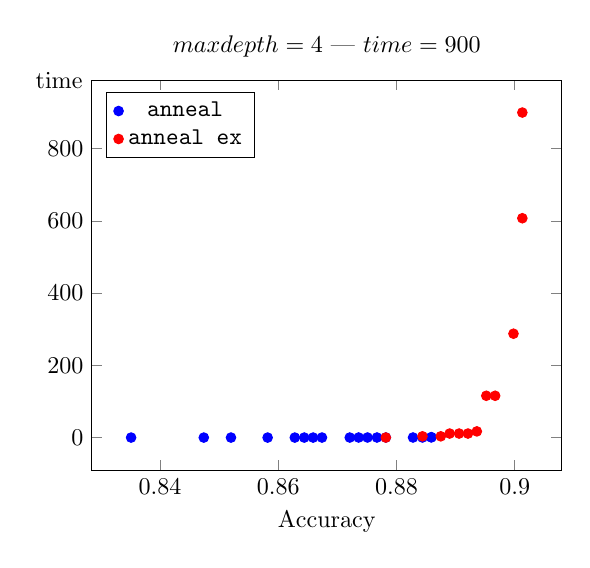
\begin{tikzpicture}[scale=0.87]
            \begin{axis}[
                title={$maxdepth=4$ | $time=900$},
                xlabel={Accuracy},
                ylabel={time},
                every axis y label/.style={at={(-0.07,1)}},
                legend pos=north west]
            \addlegendentry{\texttt{anneal}}
            \addplot [only marks, blue, mark=*]
            table[meta=label] {
            x y label
            0.8351 0 a
            0.8474 0 a
            0.852 0.003 a
            0.8582 0.006 a
            0.8628 0.006 a
            0.8644 0.006 a
            0.8659 0.011 a
            0.8674 0.101 a
            0.8721 0.101 a
            0.8736 0.188 a
            0.8751 0.2 a
            0.8767 0.203 a
            0.8782 0.203 a
            0.8828 0.205 a
            0.8844 0.205 a
            0.8859 0.53 a
            0.8859 1.162 a
            };
            \addlegendentry{\texttt{anneal ex}}
            \addplot [only marks, red, mark=*]
            table[meta=label] {
            x y label
            0.8782 0.082 a
            0.8844 3.464 a
            0.8875 3.469 a
            0.889 11.16 a
            0.8906 11.17 a
            0.8921 11.17 a
            0.8936 17.12 a
            0.8952 115.8 a
            0.8967 115.8 a
            0.8998 287.7 a
            0.9013 607.5 a
            0.9013 900.2 a
            };
            \end{axis}
        \end{tikzpicture}
        \qquad
        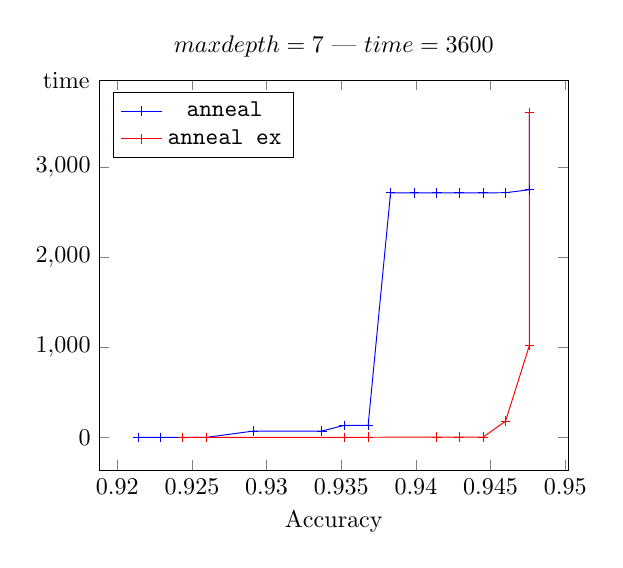
\begin{tikzpicture}[scale=0.87]
            \begin{axis}[
                title={$maxdepth=7$ | $time=3600$},
                xlabel={Accuracy},
                ylabel={time},
                xticklabel style={/pgf/number format/.cd,fixed,precision=3},
                every axis y label/.style={at={(-0.07,1)}},
                legend pos=north west]
            \addlegendentry{\texttt{anneal}}
            \addplot [blue, mark=+]
            table[meta=label] {
            x y label
            0.9214 1.844 a
            0.9229 1.849 a
            0.9244 1.973 a
            0.926 2.972 a
            0.9291 72.27 a
            0.9337 72.27 a
            0.9352 136 a
            0.9368 136.2 a
            0.9383 2710 a
            0.9399 2711 a
            0.9414 2711 a
            0.9429 2711 a
            0.9445 2711 a
            0.946 2713 a
            0.9476 2746 a
            0.9476 3601 a
            };
            \addlegendentry{\texttt{anneal ex}}
            \addplot [red, mark=+]
            table[meta=label] {
            x y label
            0.9244 0.098 a
            0.926 3.038 a
            0.9352 3.049 a
            0.9368 3.743 a
            0.9414 5.168 a
            0.9429 5.173 a
            0.9445 5.584 a
            0.946 181.5 a
            0.9476 1021 a
            0.9476 3601 a
            };
            \end{axis}
        \end{tikzpicture}
    \end{center}
    \caption{\texttt{anneal} vs \texttt{anneal ex} performance}
    \label{fig:annealperf}
\end{figure}

\paragraph{} The left chart in figure \ref{fig:annealperf} confirms what we have already established although in this
case, the CPU time skyrockets with barely any accuracy gain. In order to find how this method scaled to deeper trees,
we used the same datasets and we ran a one hour search with a maximum depth of 7 which is represented on the right chart
of figure \ref{fig:annealperf}. The two datasets end on the same accuracy after one hour however, the expanded dataset
provides very quickly an accuracy close to what is obtained at the end of the execution whereas the accuracy for the
normal dataset is far slower to increase.

\paragraph{} Acquiring better accuracies faster by almost a factor of two for deeper trees might be a significant
advantage when using the extended datasets which produce multivariate decision trees. It is very important to note
that for this specific case, we only tested the \texttt{anneal} dataset so a lot more testing would be needed to confirm
this.

\newpage

\section{Limits}
\paragraph{} We said our dataset expansion script was not meant to be used with massive datasets but it can still
be utilized. The current implementation works in a way that the dataset is saved into the memory and the changes are
made in the memory; when all the new features are added, we write the new dataset to a file. This obviously does not
scale very well for bigger datasets unless we have enough RAM. We focused on the results rather than the optimization
of our script but it would be very easy to fix this issue. Instead of writing the file when the dataset is complete,
we can simply write it line by line. This is to be done during the second part of the master thesis.

\paragraph{} On the side of the actual results we got, even though we have an improvement when using expanded datasets,
the small accuracy gain can be considered negligible or even anecdotic. It would be interesting to try using datasets
specifically benefiting from multivariate decisions. Regardless of the datasets used, further testing is needed using
different depths and longer execution times.



\chapter*{Conclusion}
\paragraph{} In a nutshell, we went over the basics of decision and multivariate decision trees, explaining some core
principles and important classification algorithms in a brief state of the art. Our work so far lead us to develop
a Python script taking any binary dataset and expanding it with new features that are conjunctions of the original
features. We tested this additionnal preprocessing step using the \texttt{Blossom} optimal decision tree classification
algorithm and obtained multivariate decision trees with slightly better accuracies than their univariate counterparts.
Even though this is a minor improvement, equivalent accuracies to those found with untouched datasets are found earlier
in the research. Finally, we identified several refinements to make to our script and testing methodology as well as
new possible leads to follow during the second part of the master thesis.



\nocite{*}
\bibliographystyle{unsrt}
\bibliography{references}



\appendix
\chapter*{Appendix}
The code of our expansion script, the traces of the \texttt{Blossom} alogorithm for our tests as well as the code for
this report can be found on \href{https://github.com/Selarow/blossom}{GitHub}.


\section*{Experimental results}
All the test accuracy tables can be found below.\\
\it Benchmarks done using Intel(R) Core(TM) i7-1165G7






\end{document}